\section{Component Densities}

\begin{figure}[h!]
\begin{center}
	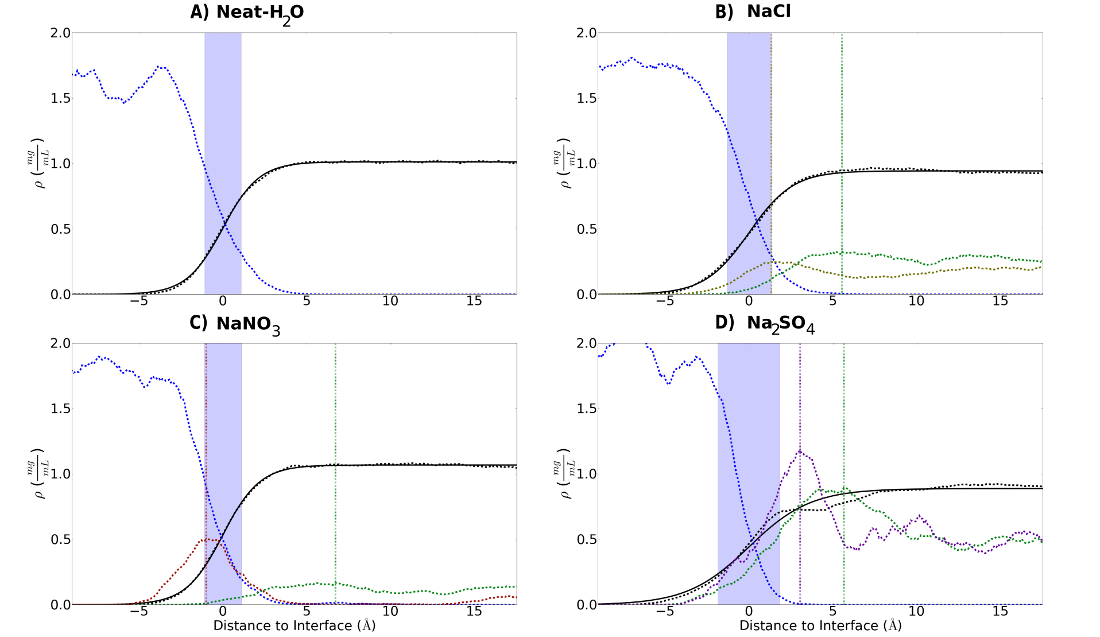
\includegraphics[scale=1.0]{images/densities.png}
	\caption{Aqueous salt solution (1.2 M) and CCl$_4$ surface density profiles. (A) Neat-\ctcwat, (B) NaCl, (C) NaNO$_3$, and (D) Na$_2$SO$_4$ aqueous solution densities are plotted with the water-oxygen density (dashed black) and the corresponding fitted lineshape (solid black). The CCl$_4$ (dashed blue), Na$^+$ cation (dashed green, scaled 10x) and respective anion (scaled 5x) densities are also shown for each system. The maxima of the ionic components are marked with dashed vertical lines of the same colors.}
	\label{fig:density-plots}
\end{center}
\end{figure}

The component density profiles of each system were calculated to study the effects of added salts on water's density profile, and to find any deviations in the behavior of water from the \ctcwat system. The water density profile of each system was fitted to a hyperbolic tangent function (Eq. \ref{tanh_fit}). The resulting plots are shown in Figure \ref{fig:density-plots}. The profiles were centered about the GDS locations, $z_0$, at 0.0\angs, and all lineshapes are plotted as distances to the GDS. Each interfacial width, $d$, is designated as a highlighted blue region of width $d$ centered about $z_0$. The widths of the interfacial regions for the neat-\ctcwat (A), NaCl (B), NaNO$_3$ (C), and Na$_2$SO$_4$ (D) systems are 2.16, 2.62, 2.20, 3.69\angs, respectively. In each of the salt solutions, the anion density profile shows higher density near the interface, appearing as a peak in the density profile. These anion enhancements all occur closer to the interface than the corresponding counter-cation density enhancement. Various parameters of interest such as the interfacial thicknesses, ionic enhancement locations (taken to be the location of the maxima in the ion profiles), and relative distances between the peaks of the ion profiles are collected in Table \ref{table:double-layer}.

\begin{table}[htdp]
	\begin{center}
	\begin{tabular}{|c||c|c|c|c|}
		\hline
		System & $d$ & Anion & Cation & Anion-Cation Distance \\ \hline
		Neat-H$_2$O & 2.16 & - & - & - \\ 
		NaCl & 2.62 & 1.33 & 5.53 & 4.20 \\
		NaNO$_3$ & 2.20 & -0.99 & 6.71 & 7.70 \\
		Na$_2$SO$_4$ & 3.69 & 3.04 & 5.64 & 2.60 \\
		\hline
	\end{tabular}
	\end{center}
	\caption{Aqueous salt system density parameters. Interfacial widths, $d$, and the locations of the maxima of the density profiles for each ionic component are listed for the simulated salt systems. The relative distances between the anion and cation density peak locations are listed to show how the different anions affect the relative location of their cationic counter-ions.}
	\label{table:double-layer}
\end{table}

The oscillations in the surface density profiles of water and the adjoining organic \ctc liquid phase have been noted previously and attributed to thermal capillary waves on a larger length-scale than the simulated system size.\cite{Chang1996} The same work also made note that the interfacial thickness is size-dependent on the interfacial surface area. Increasing the surface area dimensions should therefor cause a proportional increase in the interfacial width. As a consequence, care must be taken when making quantitative comparisons between widths and locations found in differing simulation studies. However, relative width ordering between similarly-sized systems should remain, as shown in two separate works on the \ctcwat surface.\cite{Chang1996,Hore2008}

In comparing the three salt solutions studied here, any differences in these systems are the result of the anion because the same cation was used in each system. \nacl is the simplest of the three salts with a monatomic and monovalent anion. The peak of the anion density profile is within the aqueous phase (i.e. it is found on the aqueous-side of the interfacial width). The location of the cation density peak is, as mentioned above, deeper into the aqueous phase than the anion by over 4\angs. This layering of ions within the aqueous phase is attributed to the break in the isotropy of the field of the bulk region upon introduction of the organic phase. From our studies it is clear that polarizable monovalent anions move towards the interface and effectively screen the induced field from the organic phase. The counter-ions then are drawn towards the negative charge built up by the anions to create the second ion density peak deeper in the aqueous phase. The overall shape of the water profile in the \nacl system is relatively unaffected (compared to the reference \ctcwat system Figure \ref{fig:density-plots}a) by the presence of the ions. The width of the interface is slightly increased above that of the reference system.

%In an MD study by Wick and Dang\cite{Wick2007a} of \ctcwat interfaces, larger and more polarizable monovalent anions exhibited a smaller density enhancement when compared to the \airwat interface. The \ctcwat interface was found to be a less favorable solvation environment for the more polarizable anions. 

%A break in the isotropic environment around the ions causes them to be less solvated and come in greater contact with the \ctc phase. The ions are thus pushed further into the aqueous bulk and more hydrated than at an air-interface. However, the surface activities and ion density enhancements of the more polarizable anions (i.e. I$^-$, Br$^-$) remain greater than that of a smaller and less polarizable one (i.e. Cl$^-$) at both interfaces. 
%Few surface-specific experimental analyses (i.e. SFG) have been performed on these \ctc systems and were mostly limited to the \airwat surface.

It is important to note from our density calculations that ions that increase the interfacial width at the \ctcwat interface correspond to ions that result in an enhancement of the SFG signal from interfacial water. As discussed later, our SFG calculations show excellent agreement with experimental results that also show this enhancement for such ions. Also, we find those ions that are best known to enhance the strength of hydrogen-bonding (i.e. \sul) produce wider interfaces with greater water penetration into the \ctc phase.

The \sodnit system introduces the monovalent, polyatomic nitrate anion. In our simulation we find a strong surface density enhancement of the nitrate anion as shown in Figure \ref{fig:density-plots}(c). The nitrate density peak is located the furthest out from the aqueous phase of the three salt systems. The location of the sodium cation peak in this system is a significant distance further into the bulk water relative to the anion than in either of the \nacl or \sodsul systems. The increase in ion-pair distance is likely the result of strong screening of the interfacial field by the surface-active anion, and the solvating waters around it. The interfacial width of the \sodnit system is the narrowest relative to the other salts in this study. It is likely that slight reorientation of the surface waters near \ctc enhance the solvation of the \nit in the plane of the interface and establish a much more hydrated region for the anion to adsorb. Water reorientation is more fully described later in this work. The subsurface waters then continue to screen the charge of the surface-active \nit, and decrease the coulombic force pulling the cation closer to the surface. 

%Water's ability to extend into the organic phase is affected by its hydrogen-bond network strength. Nitrate acting to break the surface water bonding thus decreases the width of the water penetration into the organic phase. 

The widest interface is that of the \sodsul solution, indicating that the \sul anions act to increase the number of interfacial water molecules on both sides of the GDS, consistent with the highly solvated nature of \sul and its larger size. \sul density enhancement (the peak of the anion density profile) is furthest into the aqueous bulk of the three anions simulated. The calculations suggest that the divalent and highly polarizable nature of the \sul anion attracts its counter-ion closest, leading to the narrowest sub-surface ionic double-layer. This attraction is likely coulombic. Although the greatest anionic concentration enhancement is further into the bulk water region, seemingly outside the region designated by the interfacial width, the water interfacial width is still greatly enhanced. This is in agreement with the experimental \sodsul SFG studies where sulfate ion leads to an enhanced SFG signal throughout the bonded OH stretch region, consistent with a larger interfacial width.\cite{McFearin2009}

%Unlike the monovalent ions, the divalent \sul anion has a very large first solvation shell and prefers a location deeper into the aqueous phase at the \airwat interface,\cite{Salvador2003} and is perhaps repelled from the interfacial region.\cite{Gopalakrishnan2005} This more highly-solvated anionic behavior coincides with the \ctcwat system seen here. Although the presence of the \ctc changes the interfacial environment from that of the \airwat interface, the field established by the deep aqueous-side location of the \sul anion density enhancement acts to affect the interface from a greater distance. 

The results of these and related simulations of ions at liquid-liquid interfaces, and the recent experimental results of similar systems demonstrate that some ions behave at the \ctcwat interface very differently than what has been calculated and observed at air-water interfaces.\cite{Wick2006,Wick2007a,Jungwirth2006a} The most striking example is that of the polyatomic nitrate ion which has been investigated at the \airwat interface by computer simulation,\cite{Miller2009,Thomas2007} spectroscopy,\cite{Otten2007,Schnitzer2000,Xu2009} and depth resolved X-ray photoemission spectroscopy.\cite{Brown2009} In contrast to what is observed here and in the related experimental SFG studies of the \ctcwat interface where nitrate ion shows an enhanced presence in the interfacial region, at the \airwat interface the nitrate ion shows no greater affinity for the surface than the bulk water. The large planar geometry of the \nit anion and its low charge appear to repel it from the \airwat surface where it encounters a reduced solvent cage and seeks a more hydrated solvation state. For \sul ion, experiments at both the \airwat\cite{Gopalakrishnan2005} and \ctcwat interface indicate sulfate does alter the interfacial region, consistent with what is observed in these computations. Unlike the monovalent ions, the divalent sulfate anion has a very large first solvation shell. These calculations indicate that at the \ctcwat interface it prefers a location deeper into the aqueous phase region and affects the interface from a greater distance than the other ions. The comparison of these computations with SFG experimental results will be discussed in more detail later in the paper.

% ********comparison to air-water**********
% Use this paragraph to talk about the differences with the AIR-water systems, and back it up with stuff found from calculations
%The majority of liquid surface studies examining ion behavior over the past decade have been conducted on \airwat interfaces. A recent review elucidates the convergence of data and conclusions regarding \airwat systems, paying special attention to relevant computational efforts.\cite{Jungwirth2006a} Ion behavior at liquid-liquid interfaces, however, is clearly different than these \airwat computational studies. The large polarizable and monovalent anions (\cl, Br$^-$, I$^-$) undergo concentration enhancement above bulk levels at the \airwat interface more than at the organic interface.\cite{Wick2006c,Wick2007a} 

%The behavior of molecular anions such as \nit at \airwat has been explored recently with computer simulation,\cite{Thomas2007,Miller2009} spectroscopy,\cite{Soule2007,Xu2009,Otten2007} and depth-resolved X-ray photoemission spectroscopy.\cite{Brown2009} Studies tend to agree that the \airwat surface affinity of the \nit anion is no greater than the water bulk (i.e. for large simulated systems), but conclusions differ on the extent of density depletion or enhancement. The large planar geometry of the \nit anion and its low charge appear to repel it from the \airwat surface where it encounters a reduced solvent cage, and seeks a more hydrated solvation state. In comparison the \nit does alter the \ctcwat interface with its density greatly enhanced within the surface region above bulk levels. Also, a wide ionic double-layer is established with its counter-ion left deeper in the aqueous bulk. 


%The surface enhancement calculated from MD studies, however, portrays the lower bound of the actual effect because of the reduced polarizability values used in simulations to avoid the so-called ``polarization catastrophe.'' Anionic surface enhancement occurs in both liquid-vapor and liquid-liquid simulations, but the enhancement effect is greater at the air-water interface than at \ctcwat.\cite{Wick2007a} 

%Ionic double-layers at both \airwat and \ctcwat surfaces have been documented in many of the studies already referenced. The distance between the anion and cation subsurface enhancements at the \ctcwat interface are shown in Table \ref{table:double-layer}. In an SFG experiment performed on the \airwat interface, Xu et al\cite{Xu2009} probed the vibrational modes of the \nit anion, rather than water's OH modes finding two anionic surface species. They concluded that solvation from an abundance of water at the interface weakens coulombic forces between ions, leading to greater cation-anion separation. The surface nitrate is dehydrated, and the water provides adequate shielding of the ionic coulombic interactions. We find ion double-layering at the \ctcwat interface with no contact-ion pair formation for each of the salts. Likely, this is due to the stronger reorientation of water in the presence of the organic phase, and the subsequent field-screening by sub-surface waters between the ionic layers.

%Ionic double-layers at both \airwat and \ctcwat surfaces have been documented in many of the studies already referenced. The distance between the anion and cation subsurface enhancements at the \ctcwat interface are shown in Table \ref{table:double-layer}. An SFG study by Schultz et al. using similar sodium salts noted the double-layer at the \airwat interface and attributed it to a ``displacement'' mechanism binding ions to interfacial waters, and forming contact-ion pairs. This was based on the lower-frequency OH vibrational mode found at 3150\cm, and the lack of signal change with added salts. Since then Xu et al studied this phenomena with an SFG experiment finding no ion-pairing in solution of various nitrates with divalent cations at the \airwat interface.\cite{Xu2009} The same study probed the vibrational modes of the \nit anion, rather than water's OH modes finding two anionic surface species. They concluded that solvation from an abundance of water at the interface weakens coulombic forces between ions, leading to greater cation-anion separation. The surface nitrate is dehydrated, and the water provides adequate shielding of the ionic coulombic interactions. We find ion double-layering at the \ctcwat interface with no contact-ion pair formation for each of the salts. Likely, this is due to the stronger reorientation of water in the presence of the organic phase, and the subsequent field-screening by sub-surface waters between the ionic layers.

%As compared to our experiment,\cite{McFearin2009} the \ctcwat double-layer size appears inversely proportional to the SFG signal enhancement of water OH vibrational modes. The tighter ionic double layer of the \sul system produces the greatest enhancement above the neat-\wat spectrum, and the widest double-layer of \nit decreases it markedly.

%It is reasonable to assume that this same effect may cause the greater cation-anion separation at the interface of the \sodnit system, even in the presence of the organic phase.

%Simulations of air-liquid systems have recently converged to a picture of an interface with enhanced ion concentrations for small monovalent ions,\cite{Wick2008a}little or no ionic density enhancement above the bulk levels for .\cite{ Surface-specific SFG has been used to characterize structural changes in the water hydrogen-bonding network at the air interface in the presence of various anions.\cite{Schnitzer2000} It was found that SFG signal from the interfacial waters was affected

%The neat-\airwat system has been simulated and analyzed previously,\cite{Wick2006c,Hore2008,Wick2008a} and is the benchmark for comparison to organic-\wat studies. Deviations in width of the interface from the neat-\ctcwat system can be attributed to the added ions in the solution. One work used SFG to detect structural changes in the water hydrogen-bonding network at the air interface in the presence of various anions, and found that it affects the SFG signal intensity from the interface, but could not create the anion density profile\cite{Schnitzer2000}. The same work found SFG intensity enhancement for hydrogen-bonded water following a trend of H$_2$SO$_4\ge$ HCl $>$ HNO$_3$. Comparison with an \airwat MD study complements this trend finding that the \sul concentration enhancement was found furthest into the water bulk.\cite{Salvador2003} Although the SFG studies stopped short of reporting a concentration profile, a recent X-ray photo-emission spectroscopy study was performed to specifically determine the nitrate concentration profile for the water-vapor interface, and reported the current differences of opinion between experiment and simulation.\cite{Brown2009} The XPS results showed a surface depletion of the nitrate anion relative to the bulk, similar to previous MD simulations of the same systems. Other works performed on the liquid-vapor interface found similar nitrate surface depletions.\cite{Otten2007} These help to contrast the effect of the presence of an organic phase as in the present work. 

% Use this paragraph to talk about the discrepancy between the nitrates at the air-water vs at the ctcwat. Also, add in the reference to the latest tobias/jungwirth/finlayson-pitts.

%Previous simulations found concentrations of small monovalent anions to be lower at the \ctcwat interface than at the air-liquid one.\cite{Wick2007a} Most of the recent studies on ion concentration near water interfaces have noted that large and polarizable ions will concentrate at the air surface,\cite{Petersen2005b,Pegram2006,Sloutskin2007,Eggimann2008} while small non-polarizable ions tend to be repelled. The surface enhancement calculated from those MD studies, however, portrays the lower bound of the actual effect because of the reduced polarizability values used in simulations to avoid the so-called ``polarization catastrophe.'' The enhancement of surface anions is also believed to be the cause of the subsurface cation density increase. The counter-ions are attracted to the concentrations of anions at the surface, which are in turn stabilized by the increased polarization of the water due to the distorted interfacial electric field. The affinity for the surface follows the trend of surface tension increments, $\frac{d\gamma}{dm_2}$, where Na$_2$SO$_4 >$ NaCl $>$ NaNO$_3$.\cite{Pegram2006} This also follows the Hoffmeister series trend for anions found to be the most ``structure-making'', and they are found to be density enhanced further into the interface. Our simulations for this work thus provide an interesting comparison to the \airwat research, and the analysis shows evidence that an organic phase causes changes in behavior of the surface waters.

